\chapter{\ChapterTitleScope}
\label{sec:zakres-funkcjonalnosci}


\section{Kontekst użytkowania aplikacji}

Głównym zadaniem aplikacji jest zapewnienie użytkownikom platformy
umożliwiającej rozgrywkę w~brydża. Strona internetowa aplikacji jest
przystosowana do każdego rozmiaru ekranu, z~której mógłby korzystać
użytkownik. Dzięki temu można skorzystać z~aplikacji, wykorzystując
telefon, komputer stacjonarny, laptop lub nawet telewizor. Wymagany
jest tylko dostęp do internetu.
%Aplikacja oprócz samej rozgrywki oferuje także przejrzenie
%wcześniejszych rozgrywek i~przeanalizowanie ich z~użyciem asystenta AI.

W~systemie aplikacji zdefiniowane są dwa typy użytkowników:
\begin{itemize}
  \item \textbf{zalogowany użytkownik} -- osoba posiadająca dostęp do
        funkcjonalności aplikacji,

  \item \textbf{anonimowy użytkownik} -- osoba niezalogowana, która nie
        posiada dostępu do
        % podstawowych
        funkcjonalności aplikacji.
        % Natomiast ma możliwość obserwowania trwających rozgrywek.
\end{itemize}

Funkcjonalności dostępne dla poszczególnych użytkowników:
\begin{itemize}
  \item \textbf{zalogowany użytkownik}:
        \begin{itemize}
          \item tworzenie i dołączanie do rozgrywek w brydża --
                gdy użytkownik założy lub zostanie jedynym
                użytkownikiem lobby, to staje się jego
                administratorem.
                Może zarządzać graczami znajdującymi się w~nim
                i~decydować ile graczy ma być zajęta przez asystenta AI.
          \item przeglądanie i analiza wcześniejszych rozgrywek
                z wykorzystaniem asystenta AI.
        \end{itemize}

  \item \textbf{anonimowy użytkownik}:
        \begin{itemize}
          \item obserwowanie trwających rozgrywek brydża.
        \end{itemize}
\end{itemize}

\begin{figure}[h]
  \centering
  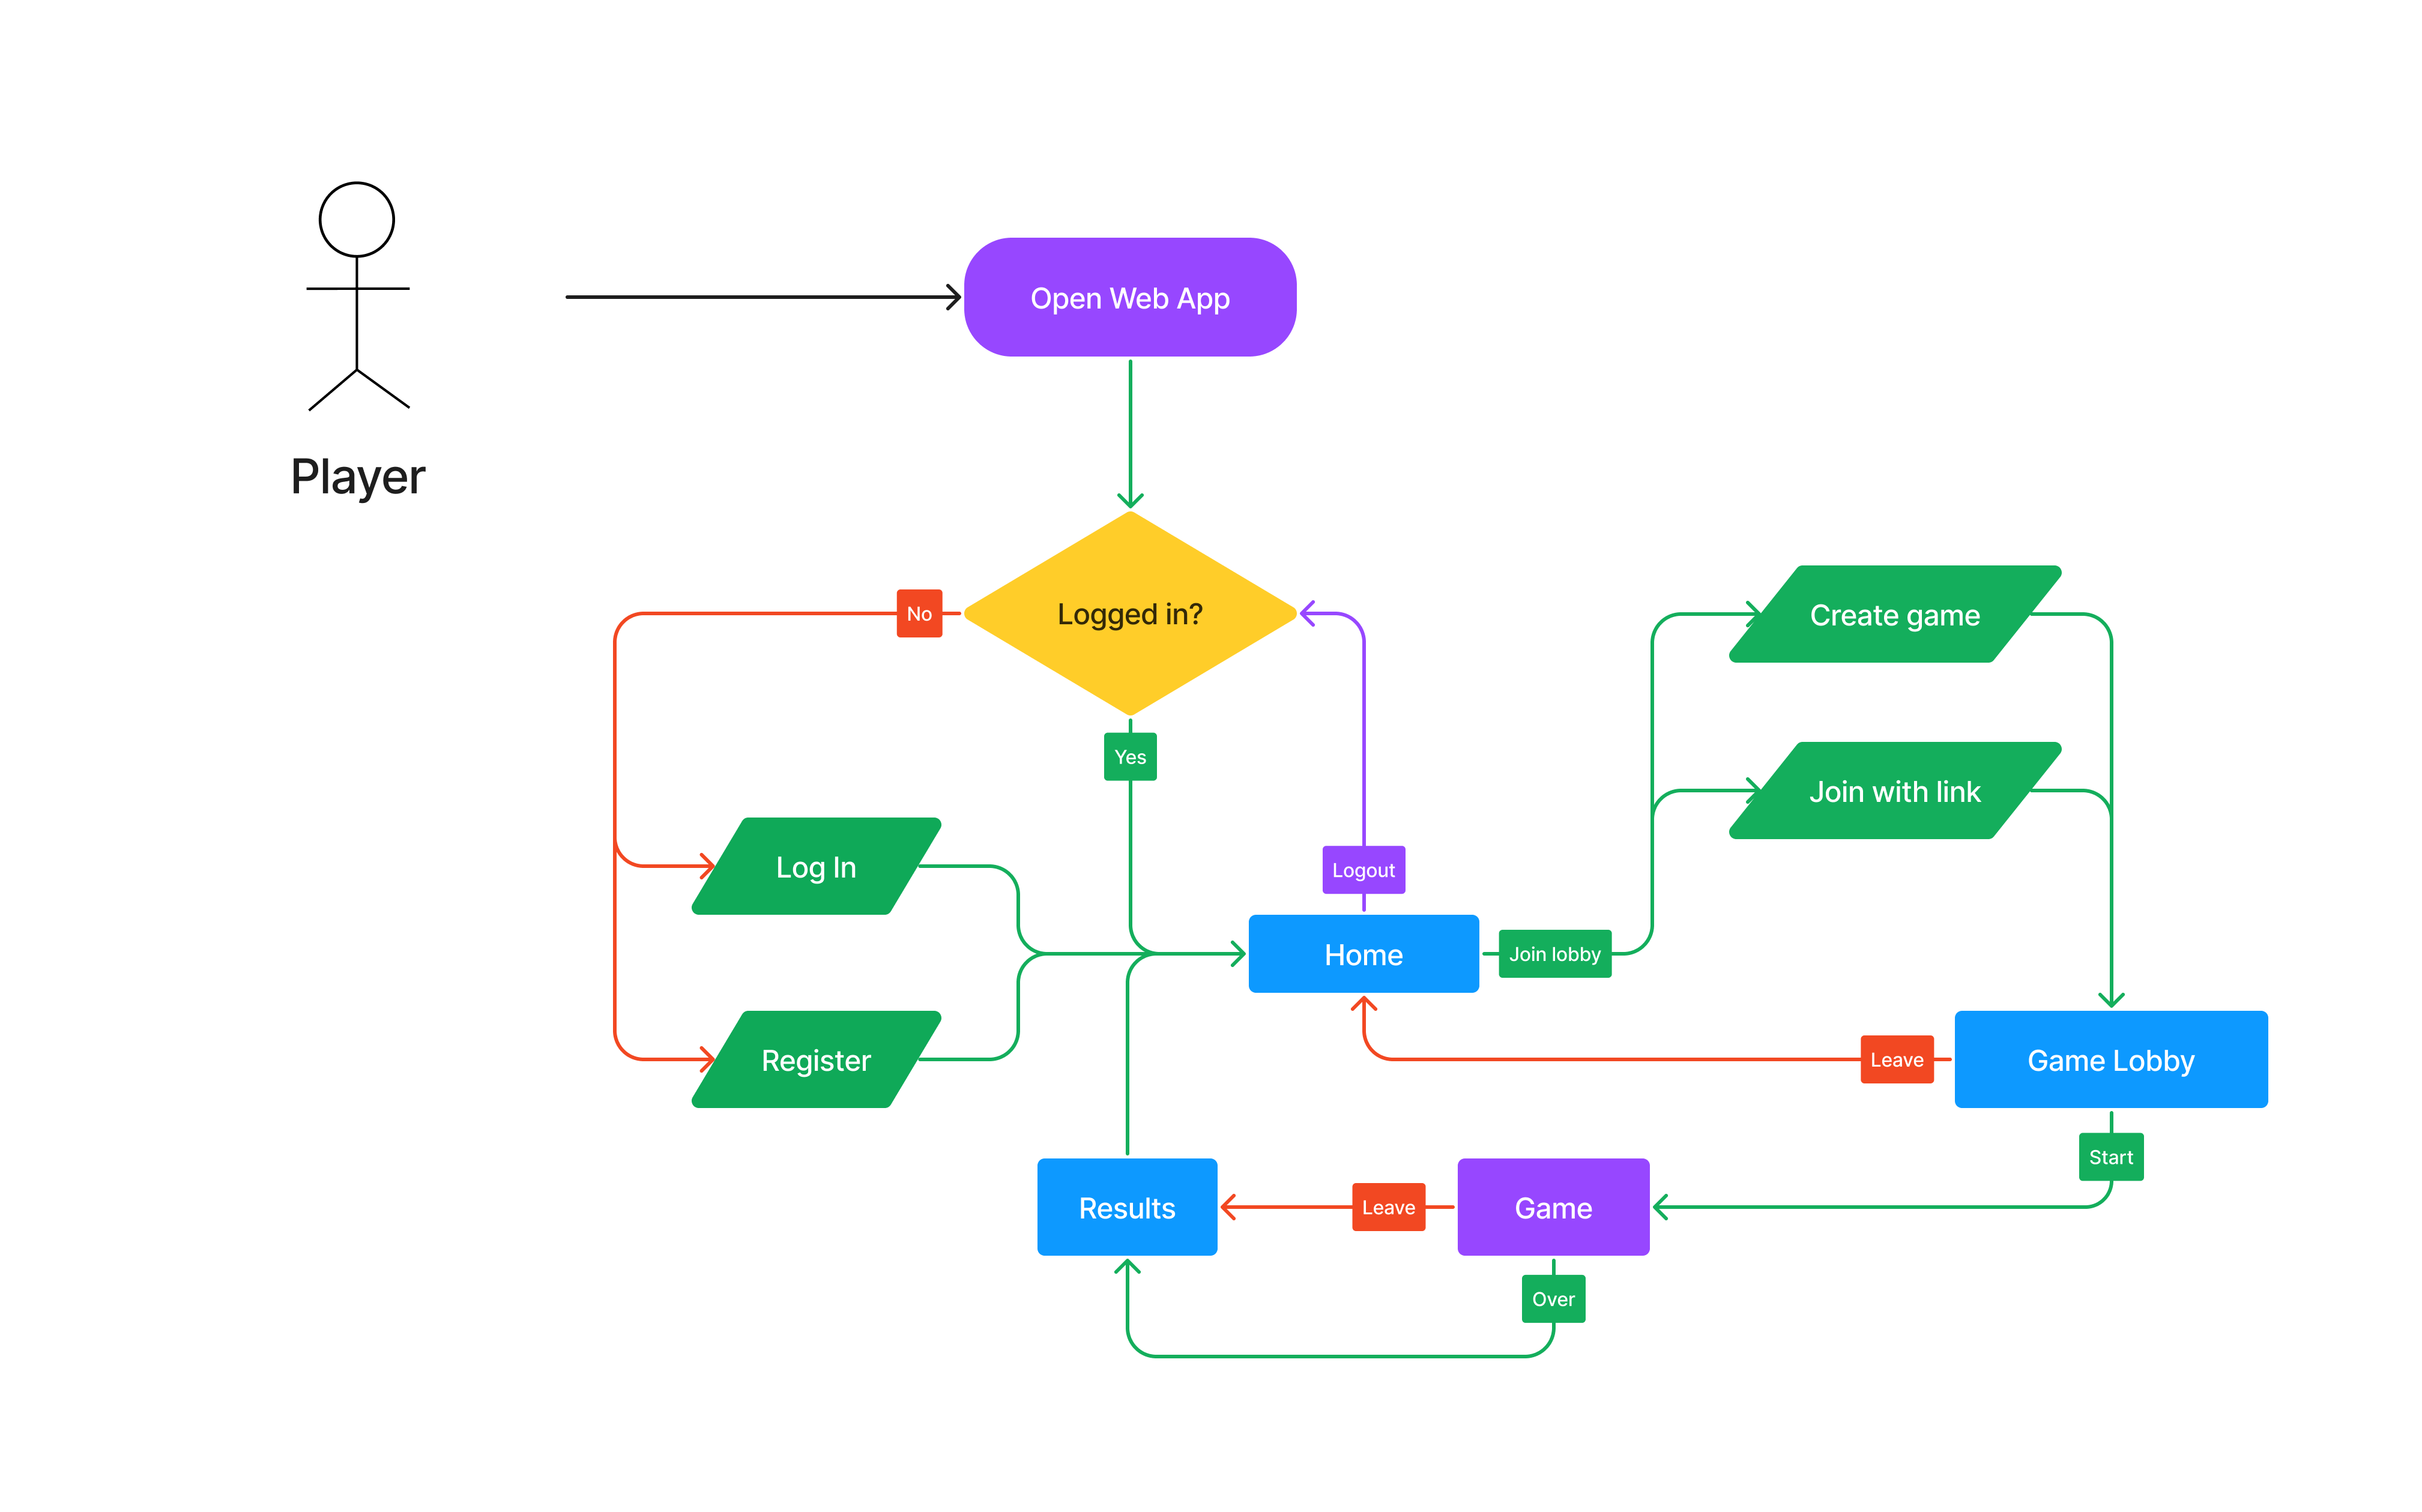
\includegraphics[width=\textwidth]{img/flow-aplikacji/user_flow.png}
  \caption{Schemat interakcji użytkownika z aplikacją}
\end{figure}

\begin{figure}[h]
  \centering
  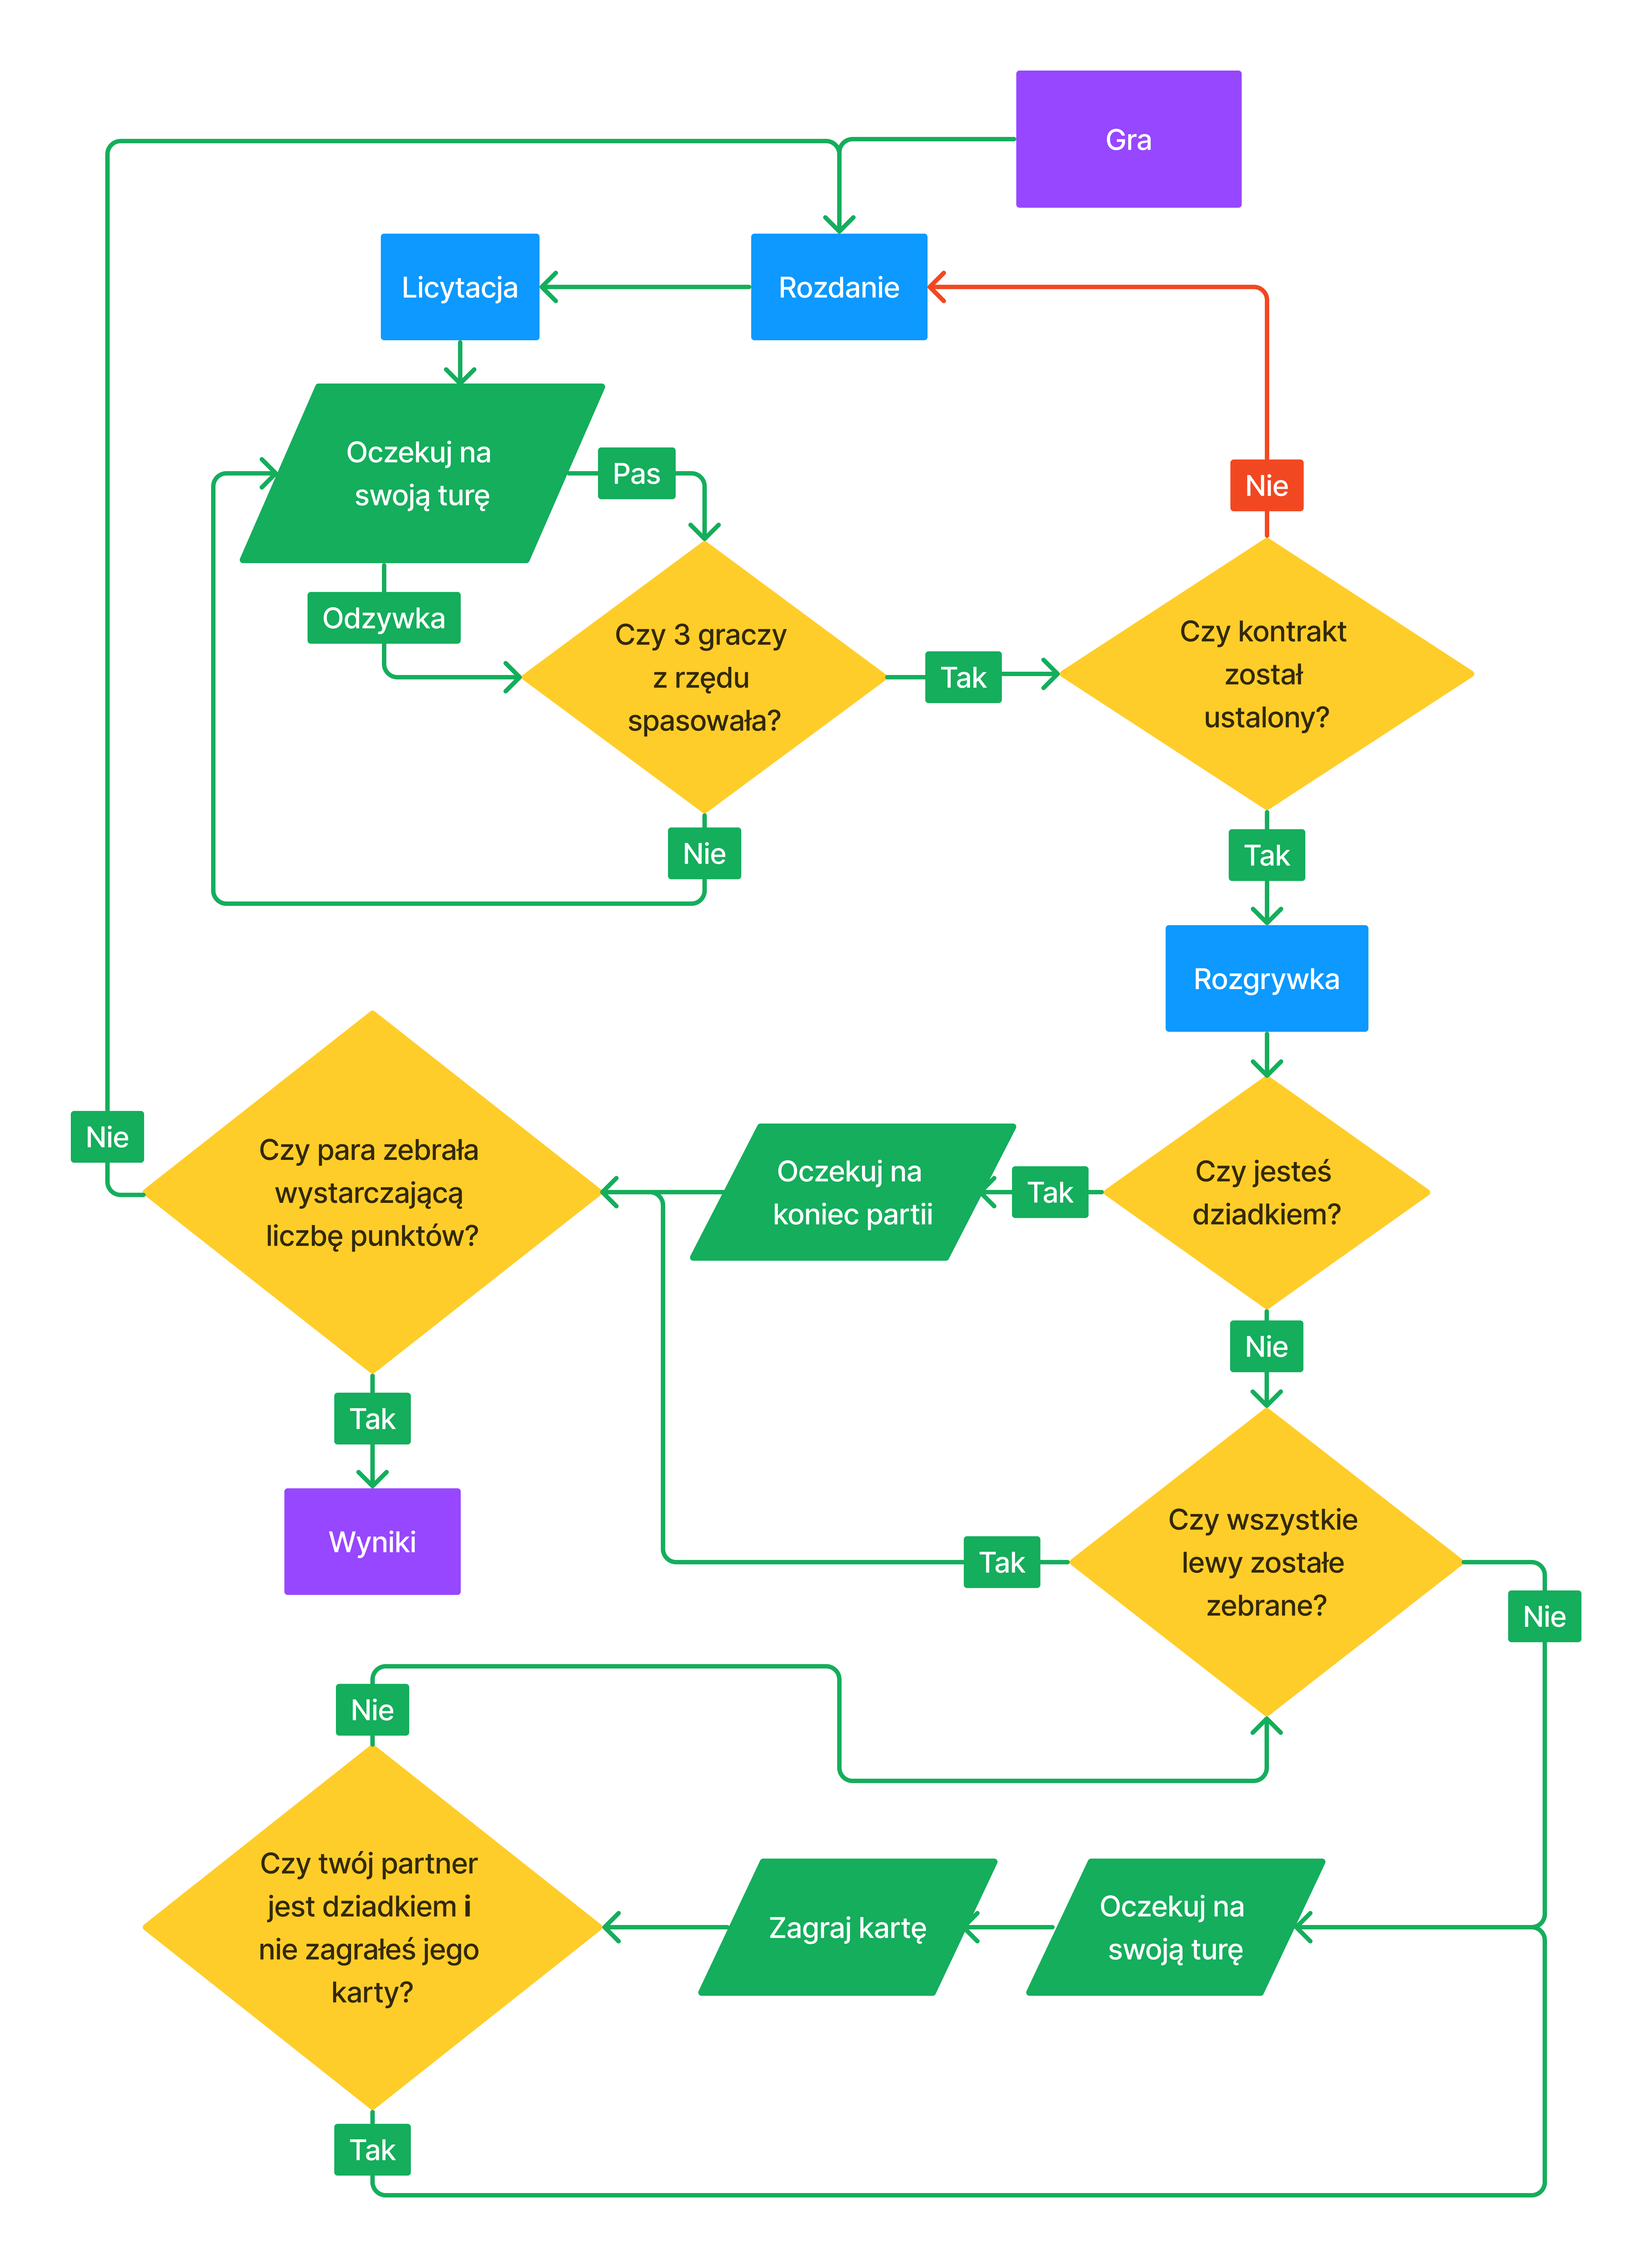
\includegraphics[width=\textwidth]{img/flow-aplikacji/game_flow.png}
  \caption{Schemat interakcji użytkownika z aplikacją podczas rozgrywki brydża}
\end{figure}

\FloatBarrier

\section{Przypadki użycia}

\subsection{Rejestracja/Logowanie do aplikacji}

Aby uzyskać dostęp do większości funkcjonalności aplikacji, wymagane
jest posiadanie konta. Anonimowy użytkownik może je utworzyć, klikając
opcję "\textbf{Register}" w~nagłówku strony. Po kliknięciu użytkownik
zostanie przekierowany do formularza rejestracyjnego.
Do utworzenia konta wymagane jest podanie własnego
pseudonimu, adresu e-mail oraz hasła. Aby uzyskać dostęp do utworzonego
konta, należy kliknąć "\textbf{Log in}" w~nagłówku strony, po czym
w~formularzu podać dane wykorzystanie podczas rejestracji.

W~przypadku nieprawidłowo podanych danych podczas rejestracji
lub logowania, błędów wynikających z~połączeniem internetowym lub
niedostępnym serwerem autentykacji użytkownik otrzyma odpowiednią
informację na ekranie.

\begin{figure}[h]
  \centering
  \includegraphics[width=\textwidth]{example-image-a}
  \caption{}
\end{figure}

\FloatBarrier

\subsection{Tworzenie lobby}

Rozpoczęcie gry w~brydża jest dostępne z~poziomu lobby. Aby utworzyć
lobby, należy kliknąć "\textbf{Create lobby}" na głównym panelu
aplikacji. Przekieruje ono użytkownika do nowego lobby
z~unikalnie wygenerowanym identyfikatorem, którego staje
się administratorem. Użytkownik może udostępnić link do adresu strony,
na której się znajduje, aby udostępnić, np. znajomym swoje lobby, do
którego mogą dołączyć.


\begin{figure}[h]
  \centering
  \includegraphics[width=\textwidth]{example-image-a}
  \caption{}
\end{figure}

\FloatBarrier

\subsection{Dołączanie do lobby}

Gdy użytkownik otrzyma link do lobby od innego użytkownika, może się
do niego dołączyć, wykorzystując adres strony lobby lub wklejając
identyfikator lobby w~odpowiednie pole w~głównym panelu aplikacji
i~klikając opcję "\textbf{Join}". W~obu przypadkach użytkownik zostanie
przekierowany do lobby.

\begin{figure}[h]
  \centering
  \includegraphics[width=\textwidth]{example-image-a}
  \caption{}
\end{figure}

\FloatBarrier

\subsection{Zarządzanie lobby}

Jeżeli użytkownik jest administratorem lub został jedynym
ludzkim graczem w~lobby, może on zarządzać graczami znajdującymi się
wewnątrz. Posiada on następujące możliwości:
\begin{itemize}
  \item usunięcie gracza z lobby -- gracz opuszcza lobby i~nie będzie
        mógł już ponownie do niego dołączyć,
  \item przyznanie pozycji w lobby jako AI -- wybrana pozycja
        gracza w~brydżu będzie kontrolowana przez asystenta AI
        i~uczestniczyć w~rozgrywce jako partner lub przeciwnik,
  \item zamknięcie lobby -- jeżeli administrator jest ostatnim ludzkim
        graczem w~lobby, opuszczenie go spowoduje jego automatyczne
        zamknięcie.
%  \item zmiana statusu lobby na publiczne/prywatne -- powoduje
%         dostępność rozgrywki rozpoczętej przez lobby w~panelu

\end{itemize}

\begin{figure}[h]
  \centering
  \includegraphics[width=\textwidth]{example-image-a}
  \caption{}
\end{figure}

\FloatBarrier

% \subsection{Obserwowanie rozgrywek}

% Gdy jakaś rozgrywka w~brydża została rozpoczęta i~ma ona status
% publiczny, jest możliwe obejrzenie jej z~panelu \textbf{Watch}.
% Z~listy publicznych rozgrywek należy wybrać interesującą i~kliknąć
% ikonę oka. 
% \end{itemize}

% \begin{figure}[h]
%   \centering
%   \includegraphics[width=\textwidth]{example-image-a}
%   \caption{}
% \end{figure}

% \FloatBarrier


\section{Specyfikacja wymagań funkcjonalnych}

% TODO

\section{Specyfikacja wymagań niefunkcjonalnych}
W naszym konceptualnym projekcie aplikacji - wirtualnego asystenta do gry w brydża, istotą jest zapewnienie nie tylko wygodnej rozgrywki, ale także niezawodnego połączenia dla wszystkich uczestników. Uniknięcie sytuacji utraty połączenia lub braku synchronizacji między graczami jest niezwykle istotne. W tym podrozdziale przedstawiamy wymagania niefunkcjonalne aplikacji, które są równie ważne jak wspomniane wcześniej wymagania funkcjonalne.
\subsection{Dostępność}
Rozwijany przez nas wirtualny asystent do gry w brydża jest aplikacją webową. Dzięki temu będzie on dostępny zarówno dla użytkowników Windows, MacOS, Linux, czy innych systemów operacyjnych. Co więcej, starannie zaprojektowane interfejsy użytkownika (UI) zostały dostosowane tak, aby były wygodne i funkcjonalne nawet na urządzeniach o niewielkich rozmiarach ekranu, umożliwiając płynne korzystanie z aplikacji nawet na urządzeniach mobilnych.
\subsection{Użyteczność}
% TODO
